\chapter{LPWAN e Lora}
Nel seguente capitolo si approfondirà il concetto di reti \emph{LPWAN} e la loro 
struttura. Si analizzeranno i principali vantaggi che queste reti portano e i
vari use-case, focalizzando l'attenzione sualla tecnologia Lora sviluppata da
Semtech. 

\section{LPWAN}
Tra le varie tipologie di rete emergenti per l'IoT, LPWAN sta riscuotendo sempre
più interesse. Questo tipo di reti si basano su una topologia a stella, la quale
permette di avere un elevato numero di devices connessi ad una sola stazione
base. Ideate per comunicazioni a lungo raggio , risultano  ideali per 
per i vari \emph{use-case} del internet of things quali smart-city, agricoltura,
assistenza sanitaria ecc... 
I  principali concorrenti che implementano queste tecnologie sono
NWave,NB-IoT, Sigfox\tm e Semtech\tm possessore di Lora\tm. 
Tra i principali competitors, Sigfox e Lora sono le tecnologie maggiormente
utilizzate.  L'implementazione proposta da Sigfox utilizza un tipo di
comunicazione basata sulle frequenze ISM e modulazione Ultra Narrow Band.
Questa tecnologia è capace di inviare messaggi con payload lungo 12 \emph{byte} 
in 6 secondi usando una frequenza di 100[Hz]. Per via della modulazione scelta e le
varie regolazioni delle frequenze ISM, utilizzando la tecnologia Sigfox si ha un
numero limitato  di 140 messaggi per giorno.
Al contrario la tecnologia Lora, implementa una modulazione basata su uno
spettro diffuso il quale permette una maggiore ricezione andando ad influire sul
data-rate possibile

\begin{figure}[h]
\centering 
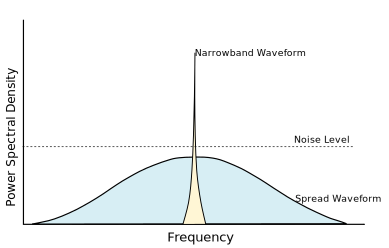
\includegraphics[width=11cm]{spread_spectrum_temp}
\caption{Comparazione tra UNB e SSP}
\end{figure}

\section{LoRa}
\emph{Lora} è una tecnologia di modulazione wirelless semi-proprietaria 
sviluppata da Semtech. Lora è composta da un layer fisico ,proprietario, che
prende il nome di \emph{Lora}\cite{LoRaCss101}  , e una parte libera chiamata 
LoRaWAN\cite{LoRaWAN101}, la quale definisce un protocollo di communicazione, 
il quale usa LoRa come layer fisico. 
I punti chiave dei questa tecnologia, sono il grande raggio di copertura e il 
basso consumo energetico per effettuare uno scambio dati. 
Per le communicazioni , vengone utilizzata la banda ISM, grazie alle
quale è possibili costrurire una rete ,che implementa questa tecnologia, senza
possedere alcuna licenza.
\improvement[inline]{Completare e riscrivere}


\section{CSS}
Alla base del layer fisico troviamo la modulazione  Chirp Spread Spectrum (CSS), questo tipo di
modulazione della frequenza, utilizzata anche in altre applicazioni radio.
Il principio di funzionamento dei segnali \emph{CSS} si basa 
 
esempio radar ecc..\improvement{Aggiungere qualche altro esempio}.
Questo tipo di modulazione ha numerosi vantaggi quali 
\begin{itemize}
\item Uno spettro idealmente rettangolare, il quale utilizza tutta la capacità
del canale e fornisce un ottima densità spettrale di potenza rispetto agli atri
tipi di trasmissione.
\item \textbf{Segnali di tipo Chirp} possono essere sovrapposti in modo tale da
poter variare il data-rate e l'energia per bit in modo adattativo per aumentare
l'efficienza complessiva.
\item \textbf{Hanno guadagno programmabile}, il quale permette di raggiungere
distanze considerevoli mantenendo un buon SNR .
\item  \textbf{Ottima risoluzione nel asse del tempo}, quindi ottimi per coprire
lunghe distanze.
\item \textbf{Immuni al effetto Doppler} 
\item \textbf{Immuni al degenerazioni per effetto di multipath} \info{Trovare
termine per multipath}
\end{itemize}
Un segnale di tipo \emph{Chirp} assume valori compresi nella banda di frequenza
$B = [f_0,f_1]$, il suo andamento è di tipo monotono , crescente o decrescente
compreso tra le due frequenze $f_0$ e $f_1$.

\begin{figure}
\begin{subfigure}[h]{\textwidth}
\centering
\import{Images/Eps/}{Chirp.eps_tex}
\caption{Segnale Chirp nel dominio della frequenza}
\end{subfigure}

\begin{subfigure}[h]{\textwidth}
\centering
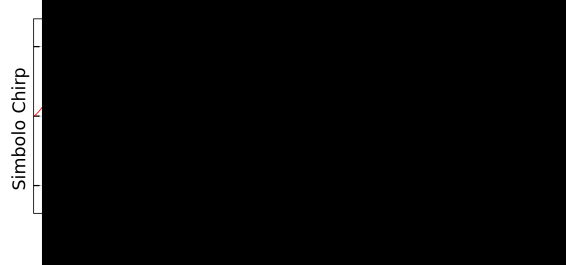
\includegraphics[width=\textwidth]{Time_Chirp}
\caption{Simbolo codificato col metodo Chirp nel dominio del tempo}
\end{subfigure}
\end{figure}

Uno degli aspetti principali del layer fisico, è la possibilità di adattare il
numero di bit codificati in un simbolo in base alle varie esigenze. Questa
possibilità\info{Riscrivere} di adattamento permette a parità di potenza di
riuscire a raggiunger distanze maggiori andando a variare, quello che nella
documentazione ufficiale è chiamato \emph{Spread Factor}. Tutto ciò significa
che (SF) rappresenta $2^{\text{SF}}$ bits in un simbolo. Un differente SF
implica anche un differente tempo di comunicazione secondo la formula
\begin{equation}
        T_s=\frac{2^{\text{SF}}}{B}.
\end{equation}

Dalla quale si evince che andando ad aumentare lo spread factor di una unità,
mantenendo una lunghezza di banda fissa $B$, otteniamo un raddoppio nel tempo di
trasmissione. Il fatto di avere messaggi più lunghi, conferisce un robustezza
superiore alle interferenze e al rumore. In discapito a tutto ciò, il fatto di
dover codificare il messaggio con un maggiore numero di simboli, aumenta la
possibilità di errore alla ricezione. 

\begin{figure}[h]
\centering 
\import{Images/Eps/}{Chirp_SF.eps_tex}
\caption{Comparazione simbolica dei vari SF}
\end{figure}

Questa nuovo modo di trasmettere i vari dati porta con se molti vantaggi.
\begin{itemize}
\item La modulazione Lora è semplice da implementare nei dispositivi, quindi i
moduli radio al loro interno saranno economici.
\item Resistente alle interferenze in banda e fuori banda.
\item Resistente  all'effetto Doppler, in questo modo è possibili utilizzare
cristalli non molto accurati al interno dei devices, in modo tale da abbattere i
costi di produzione.
\item Il modulo di ricezione è altrettanto semplice da costruire, quindi non
molto costoso.
\end{itemize}
\improvement{Rivedere i vari punti e cambiare il linguaggio}

Analizzando lo spettrogramma di una comunicazione Lora è possibili fare delle
osservazioni interessanti. 

\begin{figure}[h]
\centering 
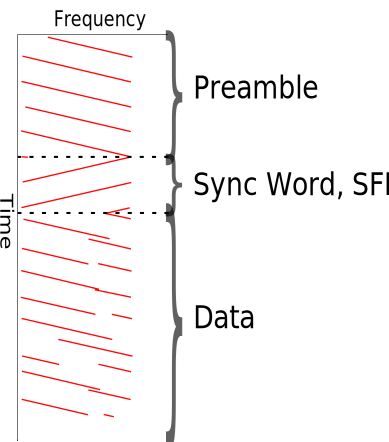
\includegraphics[width=9cm]{Chirp_Message}
\caption{Struttura pacchetto Lora }
\end{figure}

Le varie parti del pacchetto  sono facilmente determinabili, infatti e facile
vedere che il preambolo è codificato con una serie di \emph{Up-chirp}, il quale
finito inizia una serie di \emph{down-chirp} i quali determinano il SFD o Header
il quale contiene informazioni aggiuntive e possibilmente dei bit per il
controllo e correzione degli errori\unsure{Controllare header pacchetto}.
\improvement[inline]{Aggiungere immagine e finire la spiegazione}

Per quanto riguarda la struttura interna dei moduli radio, non si hanno molte
informazioni dato che la tecnologia è proprietaria di Semtech. Nella
documentazione ufficiale è presente uno schema a blocchi il quale illustra i
vari blocchi presenti al interno dei moduli radio
\begin{figure}[h]
\centering 
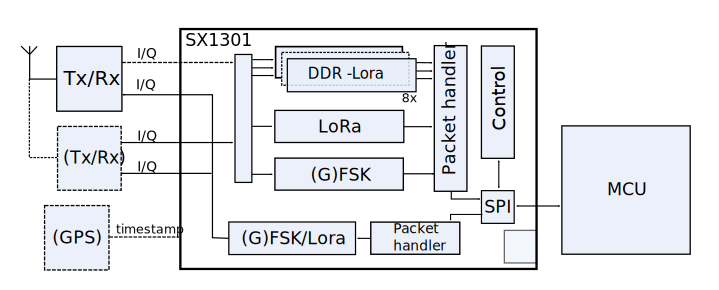
\includegraphics[width=11cm]{SX1301}
\caption{Struttura interna ricevitore SX1301}
\end{figure}
Come possiamo vedere, il gateway rimane in ascolto su 8 frequenze diverse, le
quali permettono di coprire tutti i vari SF. Tutto ciò è possibili anche grazie
al fatto che i vari SF sono quasi ortogonali fra di loro, perciò il ricevitore è
in grado di ricevere pacchetti da SF diversi contemporaneamente .Questo tipo di ricevitore può
demodulare fino ad un massimo di 8 pacchetti contemporaneamente. Inoltre questa
topologia permette di avere vari vantaggi
\begin{itemize}
\item I vari nodi della rete, possono cambiare frequenza in ogni trasmissione in
modo casuale, andando a migliorare di molto la robustezza del sistema alle varie
interferenze.
\item Non è necessario avere tabelle contenenti informazioni riguardanti il
data-rate dei vari nodi. Ogni data-rate viene demodulato contemporaneamente.
\end{itemize}
\unsure{Riguardare e aggiungere ultimo punto della documentazione pagina 14}
\section{LoRaWAN}
La parte non proprietaria del protocollo è chiamata \emph{LoRaWAN}, in essa
viene descritta la topologia di rete, la struttura dei pacchetti e le varie
classi di device possibili.

\begin{figure}[h]
\centering 
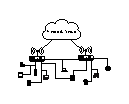
\includegraphics[width=11cm]{LPWAN_Star_network}
\caption{Struttura rete a stella LPWAN}
\end{figure}

La topologia di rete utilizzata, è una topologia a stella, nella quale molti
dispositivi sono connessi e comunicano con uno o più base station. Le BS non
sono altro che dei ponti per poter trasmettere i messaggi ricevuto dai vari
devices all Network Server, tramite una connessione ethernet, 3G o 2G. 
Per come è strutturata la rete, un messaggi inviato
da un singolo device, può essere ricevuto e inoltrato da più BS all Network
Server.

\begin{figure}[h]
\centering 
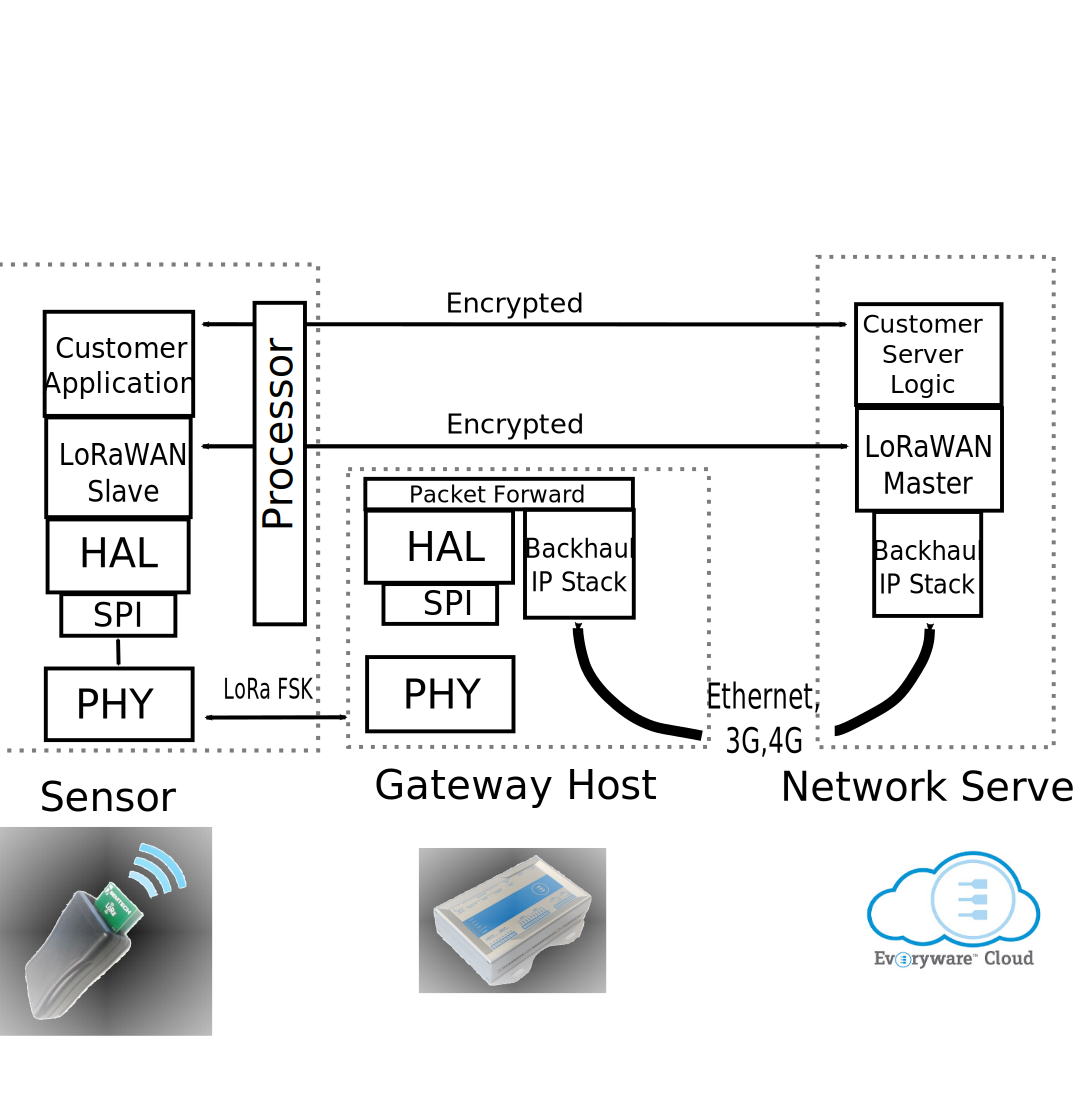
\includegraphics[width=11cm]{Lora_WAN_Stack}
\caption{Stack del protocollo della rete LoRaWAN}
\end{figure}

Il NS ha il compito di interpretare e scartare i vari messaggi duplicati che
arrivano, selezionare la BS più adatta per inviare il messaggio di downlink
creando un database di tutti i vari devices presenti nella rete 


Esistono tre classi di devices, le quali specificano i vari use-case per
possibili.
\begin{itemize}
\item \textbf{Class A} è la modalità di funzionamento predefinita. In questa
modalità il device si occupa solo di trasmettere i vari messaggi in maniera
completamente asincrona. Eseguita la trasmissione, due finestre di ascolto
vengono aperte nel end-device. La prima finestra rimane in ascolto nella stessa
frequenza in cui il dato è stato comunicato, mentre la seconda rimane in ascolto
su una frequenza nota a priori e comunicata tramite il MAC.
\item \textbf{Class B} sono devices i quali sono sincronizzati con il NS tramite
beacon packets. In questo modo hanno la possibilità di ricevere dati in un
determinata finestra di tempo. In questa classe rientrano interruttori ,
attuatori ecc..
\item \textbf{Class C} è riservata ai devices che hanno la possibilità di e
essere alimentati direttamente dalla rete elettrica, quindi possono mantenere il
ricevitore costantemente in ascolto.
\end{itemize}


